The goal of our research is to develop an automatic way to detect design and requirement \SATD comments. To do so, we first manually classify a large number of comments identifying which ones are \SATD. With the resulting dataset, we train Stanford Classifier to identify design and requirement \SATD (RQ1). Second, we inspect the features used by Stanford Classifier to identify \SATD. These features are words frequently found in comments with technical debt. We present which are the 10 most common words that indicates design and requirement \SATD (RQ2). Then, we investigate how variations in the amount of training data affects the performance of Stanford Classifier classification (RQ3). We detail the motivation, approach and present the results of each of our research questions in the remainder of this section.    

\vspace{3mm}
\noindent\rqi
\vspace{3mm}

\noindent \textbf{Motivation:} As shown in previous work \cite{Potdar2014ICSME, Maldonado2015MTD}, \SATD comments can be found in the source code. However, there is not an automatic way to identify these technical debt comments yet. The methods proposed so far heavily relies on manual examination, and there are too little evidence on how well these approaches perform and how applicable they are. We want to determine if natural language processing tools such as Stanford Classifier can help us to surpass these limitations. Stanford Classifier automatically classify comments based on specific linguistic characteristics that developers uses while writing comments. These characteristics are obtained through the training dataset that we created. For example, the training dataset can show that the adjective `ugly' is frequently found in \SATD comments. Answering this question is important to help us understand the opportunities and limitations of automatic identification of \SATD comments. 

\vspace{1mm}
\noindent \textbf{Approach:} As described in Section \ref{sec:approach}, we manually classify comments from ten open source projects into one of the following types of \SATD: design debt, defect debt, implementation debt, documentation debt and test debt. However, as shown in our previous work \cite{Maldonado2015MTD}, the most frequent \SATD comments are classified as design debt and implementation debt respectively. Therefore, in our case study we focuses our attention in these two \SATD types. 

We design our case study to test how well the maximum entropy classifier can predict \SATD comments when trained with our dataset. In order to do that, we must first prepare the training data set. The training dataset is composed by two different columns, one column is the classification and the other one is the source code comment. Then, we select all comments that were classified as not containing \SATD and the comments classified as the specific type of \SATD  that we want to predict from 9 out of 10 projects. Second, to assert the performance of the prediction we create a test dataset. The test dataset is composed by all the comments which does not contains \SATD and the specific technical debt that we are predicting from the one project that was not used in the training dataset. 

That way, if we want to classify the \SATD comments in Apache Ant project we create a training dataset using all comments from the other nine projects, namely Apache Jmeter, ArgoUML, Columba, EMF, Hibernate, JEdit, JFreeChart, JRuby and SQuirrel. Then, we use the comments of Apache Ant project to create the test dataset. Similarly with the training dataset, the test dataset possesses two columns one for the classification and other for the comment. 

Third, the classifier is executed and based on the training dataset it gives a classification for each one of the comments in the test dataset. The tool compares the classification provided in the test dataset with the predicted classification given during the execution. The results of this computation are provided in terms of precision, recall and the F1 measure achieved by the classifier.

In order to determine if the classification of the NLP tool are being effective or not we compare the obtained results with the results of two other baselines. The first one is the state-of-the-art approach in detection of \SATD comments devised by Potdar and Shihab ~\cite{Potdar2014ICSME}. This approach uses 62 comment patterns (i.e., key words) that were noticed as recurrent in \SATD comments while doing a manual inspection of 101,762 comments. The second approach used is weighed random. In fact, \SATD comments are not as frequent as comments that does not have \SATD. Through weighed random precision, recall and F1 measure is possible to show this discrepancy in the data distribution, and show how well the classifier performs compared with a random prediction.

Lastly, for each project we calculated both baselines and executed the classification process storing the results in the database to perform our analysis.

\vspace{1mm}

\noindent \textbf{Results:} We find that the predicted classification of the NLP tool greatly outperforms the current state-of-the-art approach to identify \SATD baseline and the weighed random baseline as well. Figure \ref{fig:f1_measure_comparison_design_debt} presents the comparison between the predicted F1 measure, the state-of-the-art baseline F1 measure and the weighed random F1 measure obtained during the classification of design debt. We choose to use the F1 measure to compare the approach as this measurement takes into consideration the combination of precision and recall.

It is important to notice that each one of the selected baselines for comparison has one strong point. The comment patterns approach has a high precision, but it lacks recall, i.e., this approach points correctly to \SATD comments, but it identifies a very small set of all the \SATD comments in the project. The less sophisticated weighed random baseline provides a high recall because of the two categories that we try to predicted i.e, therefore 50\% chance to randomly get one of the two classifications. 

\begin{figure}[thb!]
   \centering
  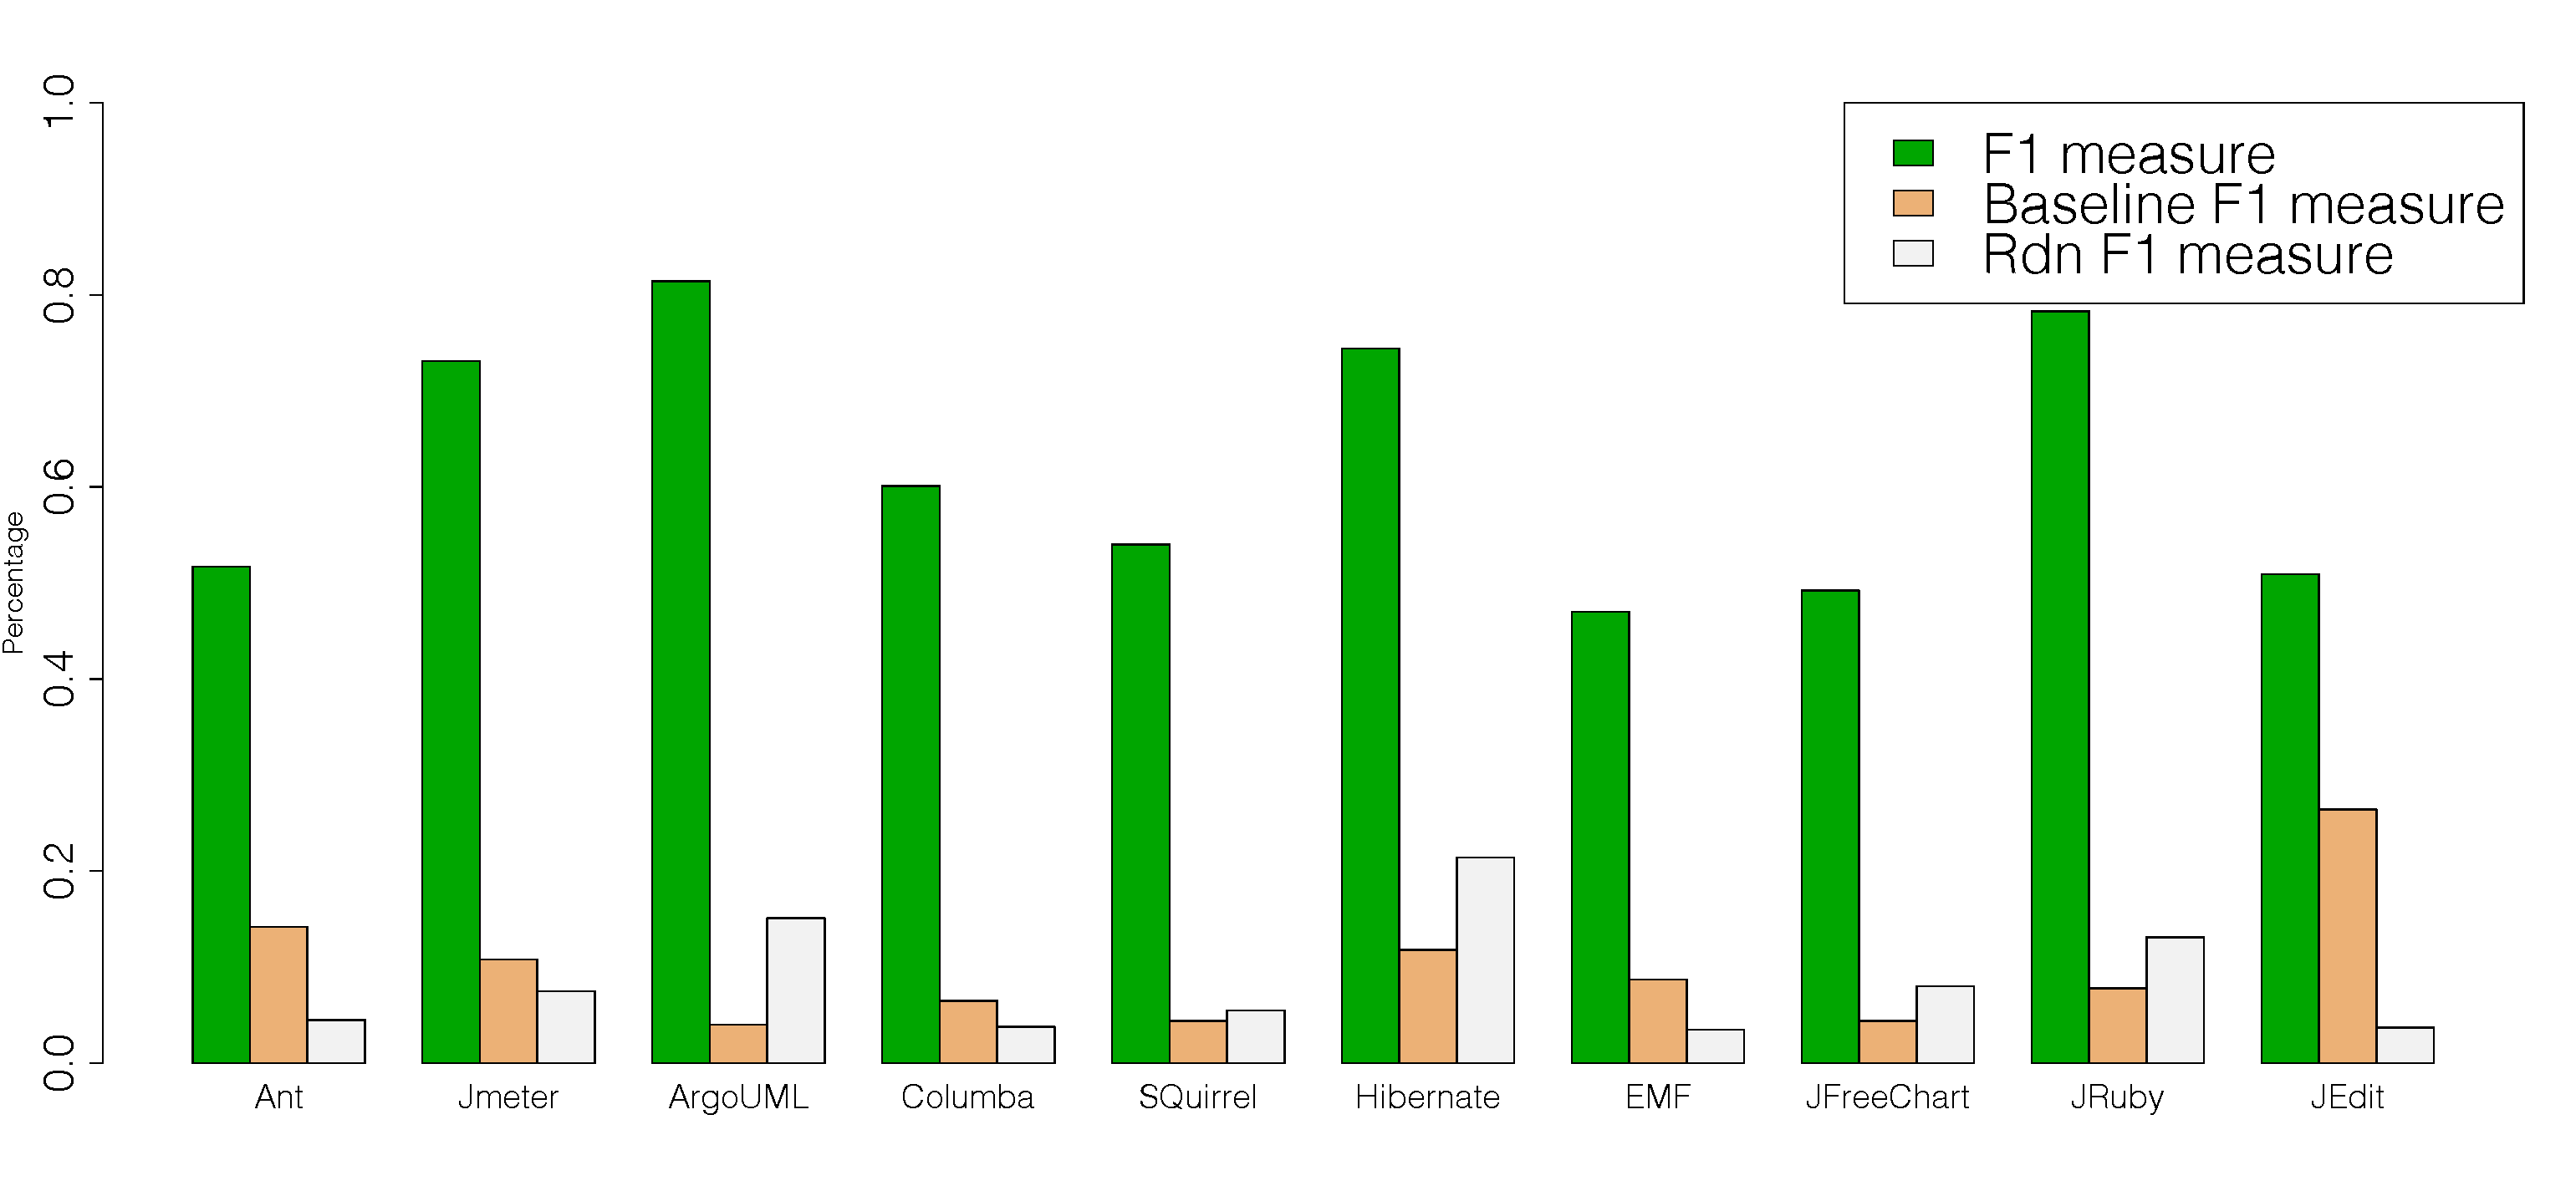
\includegraphics[width=0.48\textwidth]{figures/f1_measure_comparisom_design_2.pdf}
  \vspace{-3mm}
  \caption{F1 measure comparison Design Debt}
  \label{fig:f1_measure_comparison_design_debt}
\end{figure}

For all the projects, the F1 measure achieved by the NLP classifier is higher than the the others F1 measures. The highest F1 measure obtained for design debt was in ArgoUML with a value of 0.814. In the other hand, the lowest F1 measure obtained was in EMF with a value of 0.470. In average the F1 measure obtained was of 0.620. In comparison, the average F1 measure obtained using the state-of-the-art approach was of 0.099, and the weighed random F1 measure 0.0861. Consequently, our approach to identify design debt represent, in average, a improvement of 6 times the state of the art approach and 7 times the weighed random value. In the  Table \ref{tbl:improvement_f1measure_design} shows the improvement of our approach over the other the comment pattern baseline for each project. 
 
Similarly, Figure \ref{fig:f1_measure_comparison_requeriment} shows the comparison between the three F1 measures while identifying requirement \SATD.

\begin{figure}[thb!]
  \centering
  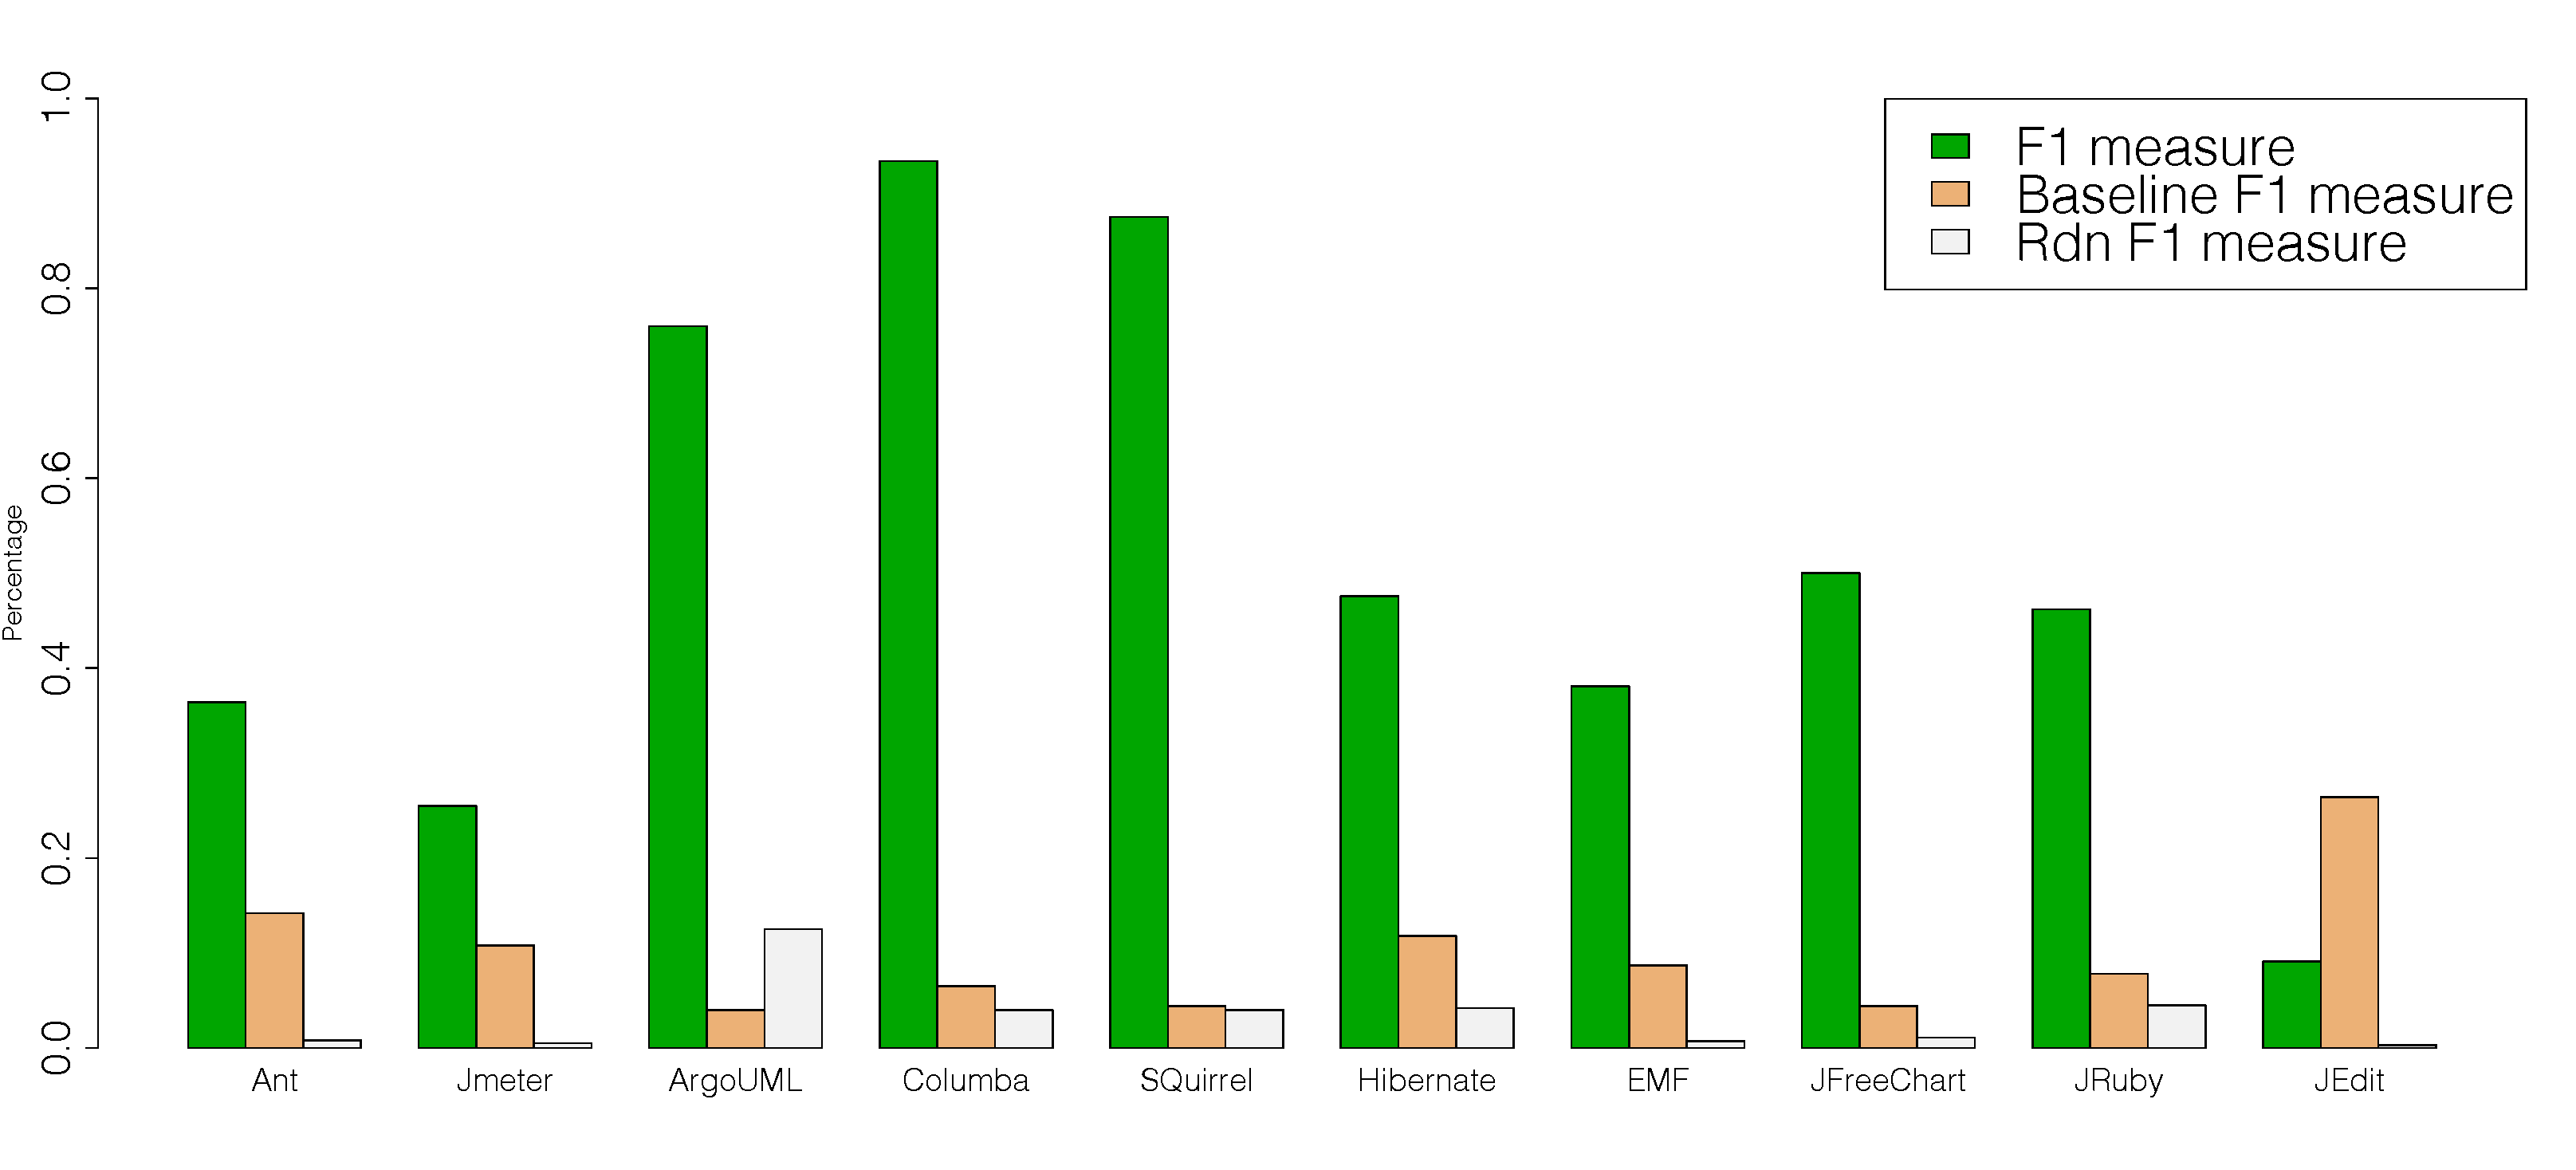
\includegraphics[width=0.48\textwidth]{figures/f1_measure_comparison_requirement_2.pdf}
  \vspace{-3mm}
  \caption{F1 measure comparison Requirement Debt}
  \label{fig:f1_measure_comparison_requeriment}
\end{figure}

We find that in 90\% of the analyzed projects the F1 measure obtained by our approach surpass the comment pattern baseline, and in 100\% of the cases we outperform the weighed random baseline. In addition to that, the comment patterns baseline calculated is the same for design debt and for requirement debt, since this approach does not distinguish between different types of \SATD as ours. 

Our highest F1 measure was on Columba with 0.934, and the lowest value was of 0.091 on JEdit. Although there was a big fluctuation between the maximum and minimum value obtained our average F1 measure was of 0.510. Despite the fact that this number is slightly lower than the average obtained while  identifying design debt, this result still impressive due the reduced amount of requirement \SATD comments that are in the projects. For example, Columba has only 134 occurrences of requirement \SATD scattered among 6,393 comments (i.e, requirement debt comments and without \SATD comments). The classifier predicted correctly 128 requirement \SATD comments (true positives), wrongly classified 12 comments as requirement debt (false positives), and wrongly classified 6 requirement debt comments as comments without \SATD (false positives). However, the classifier correctly classified 6,247 comments as comments without \SATD (true negatives).

Table \ref{tbl:improvement_f1measure_requirement} shows the improvement of our approach over the comment patterns approach. For SQuirrel the F1 measure was of 0.875 whereas the comment pattern F1 measure was of 0.044, which means that there was an improvement of 19.8 times in the identification of requirement \SATD comments using our approach. The exception is JEdit where the F1 measure was of 0.091 and the comment pattern F1 measure was of 0.264. However, we argue that using the comment patterns approach is not guaranteed that every \SATD found will be a requirement \SATD as our approach propose. Even though 0.091 is our lowest F1 measure we still outperform the weighed random F1 measured by 30 times, i.e., the weighed random F1 measure was of 0.003 for JEdit. 

\begin{table}[!hbt]
    \begin{center}
        \caption{Improvement over the random F1 measure for design}
        \label{tbl:improvement_f1measure_design}
        \begin{tabular}{l| c c c }
        \toprule
        \textbf{Project} & \textbf{F1} & \thead{Baseline\\F1} & \textbf{Improvement}\\
        \midrule
         Apache Ant      &  0.517 &  0.142  &  3.6  x\\
         Apache Jmeter   &  0.731 &  0.108  &  6.7  x\\
         ArgoUML         &  0.814 &  0.040  &  20.3 x\\
         Columba         &  0.601 &  0.065  &  9.2  x\\
         EMF             &  0.470 &  0.087  &  5.4  x\\
         Hibernate       &  0.744 &  0.118  &  6.3  x\\
         JEdit           &  0.509 &  0.264  &  1.9  x\\
         JFreeChart      &  0.492 &  0.044  &  11.1 x\\
         JRuby           &  0.783 &  0.078  &  10   x\\
         SQuirrel        &  0.540 &  0.044  &  12.2 x\\
        \bottomrule
        \end{tabular}
    \end{center}    
\end{table}

\begin{table}[!hbt]
    \begin{center}
        \caption{Improvement over the random F1 measure for requirements}
        \label{tbl:improvement_f1measure_requirement}
        \begin{tabular}{l| c c c }
        \toprule
        \textbf{Project} & \textbf{F1} & \thead{Baseline\\F1} & \textbf{Improvement}\\
        \midrule
         Apache Ant      & 0.364 & 0.142  &  2.5  x\\
         Apache Jmeter   & 0.255 & 0.108  &  2.3  x\\
         ArgoUML         & 0.760 & 0.040  &  19   x\\
         Columba         & 0.934 & 0.065  &  14.3 x\\
         EMF             & 0.381 & 0.087  &  4.3  x\\
         Hibernate       & 0.476 & 0.118  &  4    x\\
         JEdit           & 0.091 & 0.264  &  N/A   \\
         JFreeChart      & 0.500 & 0.044  &  11.3 x\\
         JRuby           & 0.462 & 0.078  &  5.9  x\\
         SQuirrel        & 0.875 & 0.044  &  19.8 x\\
        \bottomrule
        \end{tabular}
    \end{center}    
\end{table}

\conclusionbox{We find that NLP techniques, such as maximum entropy classifiers, can be used effectively to find \SATD comments. We achieved an average F1 measure of 0.62 for design debt and an average of 0.51 while classifying requirement debt. For the two types that we classify using our dataset we perform better than the state-of-the-art F1 measure average, and the weighed random F1 measure average}

\vspace{3mm}
\noindent\rqii
\vspace{3mm}

\noindent \textbf{Motivation:} After asserting the efficiency of NLP classifiers predicting \SATD we want to better understand which are the words that developers use when writing \SATD comments. Answering this question will provide insightful information that can guide future research direction and broaden our understanding on \SATD.     

\vspace{1mm}
\noindent \textbf{Approach:} As mentioned before, we use the Stanford Classifier to predict \SATD comments, and the first part of the prediction process is to generate the features (i.e., words) that will be used to classify the comments. These features, are fragments of data that possesses a class (i.e., design debt, requirement debt or without technical debt) and a weight. These features are extracted from the comments in the training dataset, and then applied to the test dataset where they are combined to reach a vote. That is, every feature that is satisfied by the comment being classified (i.e., matched) will be used to predict the class for the comment. The vote is given to the class that has more weight, therefore positive weight features that matches the comment being classified will result in a higher weight, and the class that has the higher weight will be assumed as the predicted class.

For example, given three different features: `hack' with a weight of 5.3 , `dirty' with weigh of 3.2 both for design debt and `ignore' meaning that the comment is not a technical debt with a weight of 4.1. When classifying the following comment ``this is a dirty hack and should not be ignored'', all features would have been matched, and the vote decision would be like this: design debt weight = 8.5 (i.e., feature 1 plus feature 2) and without classification weight = 4.1 resulting in a comment classified as  design debt.

For each project analyzed we collect the features used to predict the \SATD comments. These features are provided by the tool as output and stored in a text file. The features are written in the file based on the weight that it has, ordered by highest weight to the lowest weight meaning more relevant features to less relevant features respectively. Based on these files, we rank the words calculating the average ranking position of the analyzed feature across the ten different files. 

This way, we determined the top 10 features (i.e, most relevant based on the weight) for design \SATD and requirement \SATD.

\vspace{1mm}
\noindent \textbf{Results:} 
\todo{generate ranking again considering the unique top ten words for each project}
\todo{if the word is not in the list give the highest value (11)}

Table \ref{tbl:top_ten_features} shows the top 10 features for the identification of \SATD in the ten studied projects ordered by relevance. The first column we  present the ranking of the word. The second column we list the features used in the identification of design \SATD, and the third column is the list of features used to identify requirement \SATD.

\begin{table}[!hbt]
    \begin{center}
        \caption{Top ten features for Self-Admitted Technical Debt}
        \label{tbl:top_ten_features}
        \begin{tabular}{l| l l }
        \toprule
        \textbf{Order} & \thead{Design\\TD} & \thead{Requirement\\TD}  \\
        \midrule
         1  & hack       &   todo              \\
         2  & workaround &   needed            \\
         3  & kludge     &   implementation    \\
         4  & yuck!      &   fixme             \\
         5  & fixme      &   xxx               \\
         6  & todo       &   auto-generated    \\
         7  & stupidity  &   ends?             \\
         8  & ugly       &   configurable      \\
         9  & unused?    &   convention        \\
         10 & sucks      &   apparently        \\
        \bottomrule
        \end{tabular}
    \end{center}    
\end{table}

It is possible that the same feature is used to classify design debt and requirement debt. However, the weight of this feature can be different accordingly with the type being classified. As we can see in Table \ref{tbl:top_ten_features}, `FIXME:' appears in both columns although it has a higher ranking when classifying requirement debt than design debt. 

In spite of the fact that features with higher weights will have more impact during the classification the final vote is given based on the combined weight of all matching features. In average the number of features to classify design debt was of 6,196 whereas for requirement debt was of 2,889.

\conclusionbox{We find that the most common words in design \SATD comments: `hack', `workaround', `kludge', `yuck!', `fixme', `todo', `stupidity', `ugly', `unused?' and `sucks'. Whereas, for requirement \SATD comments the most common words are: `todo', `needed', `implementation', `fixme', `xxx', `auto-generated', `ends?', `configurable', `convention' and `apparently'.}

\vspace{3mm}
\noindent\rqiii
\vspace{3mm}

\noindent \textbf{Motivation:} Answering this research question will allow us to better estimate effort for future research in the area. More specifically, it will be beneficial to 1) make this kind of analysis more efficient, so manual classification of comments, that is time consuming and difficult by nature, can be kept to a minimum. 2) Helping researchers interested in applying the same technique to analyze \SATD in domains not covered in our study, another programming languages than Java, or even comments written in languages other than English. 

\vspace{1mm}
\noindent \textbf{Approach:} We executed the classification process several times with an increasing number of comments being added to the training dataset while collecting the results to analyze the changes between each iteration. 

We first select a project that will be used to create the test dataset and we keep it separated from the other nine projects. Second, we take the comments of one of the nine remainder projects to create the training dataset. Third, we run the classification process and collect the results. Fourth, we incrementally add the comments of another project to the training dataset and repeat the classification process collecting the results. 

We cycle trough this steps until we had added all nine projects comments in the training dataset. 

We apply this approach for each one of our ten studied projects classifying design and requirement \SATD comments. We ranked the projects that contained more \SATD of the specific type being classified so that they can be added first to training dataset. 

Intuitively we expect that the performance of the classifier would improve with each iteration as more comments are being added to the dataset. However, we find that this is not what always happen, and that the addition of more comments can decrease the performance of the classifier in given scenarios.

Due to that, we determined which iteration has the highest performance for each project. We called this iteration as the maximum F1 measure. To know how close the other iterations were from reaching the maximum performance we use the iteration F1 measure value to calculate the percentage of the maximum F1 measure it represents.

Lastly, for each type of technical debt classified we determined which is the iteration that is the most significant across all projects by calculating the average of the percentage of the maximum F1 measure.

\vspace{1mm}
\noindent \textbf{Results:} We find that, in the identification of design \SATD comments, the F1 measure improves significantly in the first three iterations and, after that, the improvement rate keep a more stead pace. Figure \ref{fig:design_ant_result} shows this behavior using Apache Ant as an example. For the sake of space we only provide the figure of one analyzed project, but we performed this analysis for all ten projects and Apache Ant is a good representation of our dataset. 

% the scale of the figure does not match the numbers presented fix it later
\begin{figure}[thb!]
  \centering
  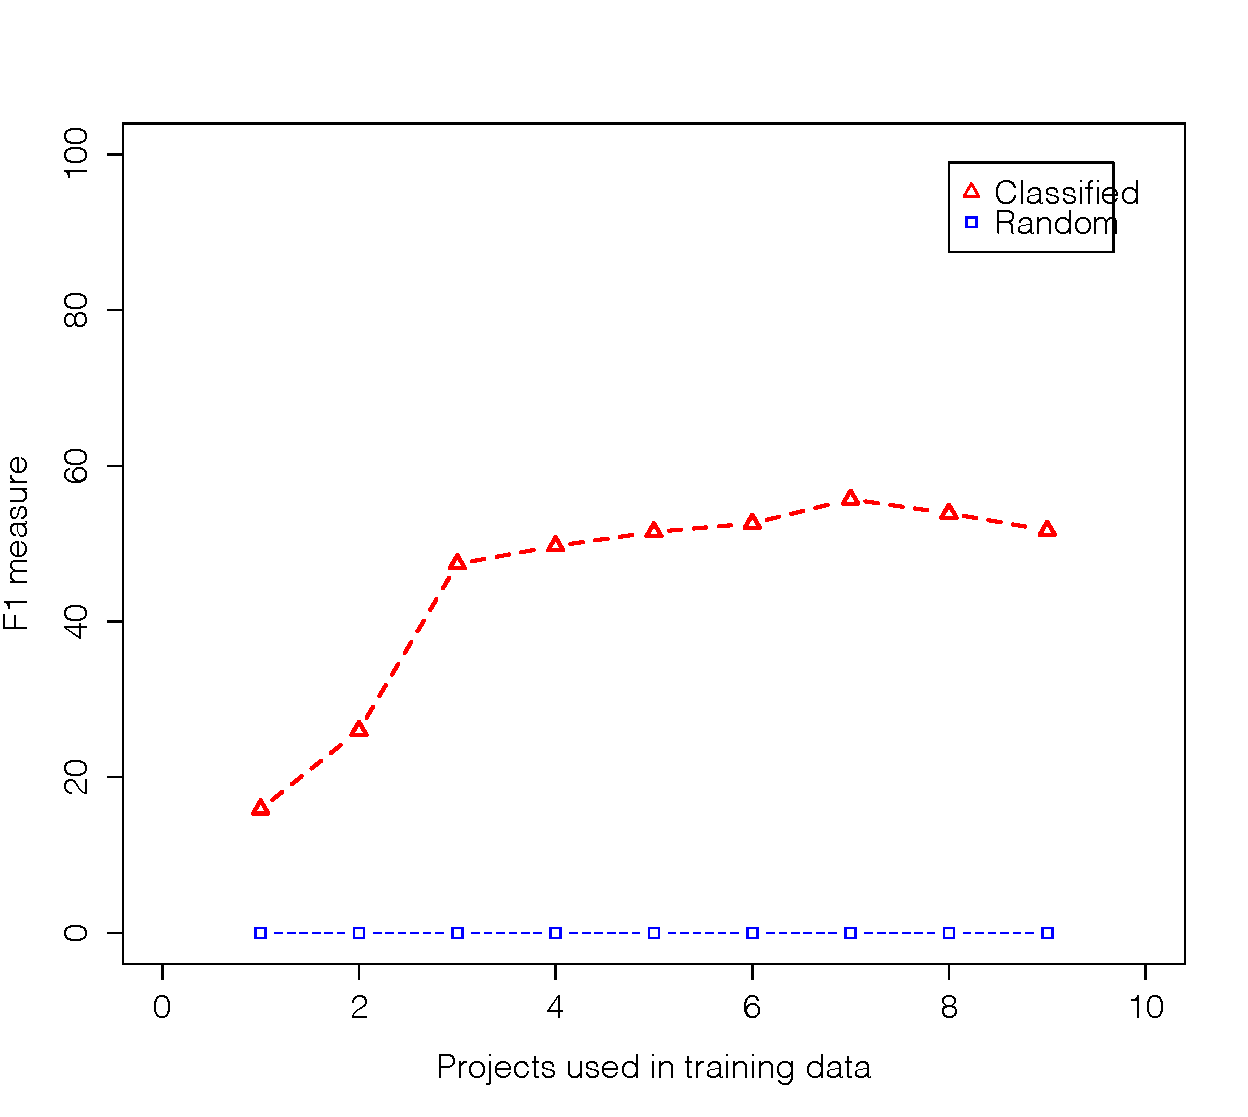
\includegraphics[width = 0.48\textwidth]{figures/design_ant.pdf}
  \vspace{-3mm}
  \caption{Apache Ant Design Debt classification}
  \label{fig:design_ant_result}
\end{figure}

The values of the F1 measure shown In Figure \ref{fig:design_ant_result} are in order execution: 0.159, 0.260, 0.474, 0.497, 0.515 ,0.526 ,0.557 ,0.539 and 0.517.

Analyzing Apache Ant, we notice that it has a F1 measure of 0.474 in the third iteration and 0.557 in the seventh iteration, which is the maximum F1 measure achieved for the project. The F1 measure achieved in the third iteration represents 85\% of the maximum F1 measure achieved in the seventh iteration, and this percentage was reached using 1,499 comments whereas the maximum F1 measure used 2,404 comments in the training dataset. Therefore, for Apache Ant we could achieve 85\% of the maximum result using only 62\% of the comments. Therefore, we find that the third iteration provides a good trade off between prediction performance and number of comments to create the training dataset.

Analyzing the evolution of the F1 measure through the iterations we notice that there are drops in the performance even with the addition of more comments in the training dataset. Therefore, we analyzed the iterations individually to determine which iteration performs better. Based on the average of the percentage of the maximum F1 measure we find that the best performance of the classifier is achieved during the eighth iteration when identifying design \SATD comments. 

At the eighth iteration the average of the maximum F1 measure is of 96.57\% using in average 2,353 comments to create the training dataset. In comparison, the ninth iteration have an average of the maximum F1 measure of 95.99\% which is slightly lower than the average obtained in the eighth iteration, and uses more comments in the training dataset (i.e., 2,432). 

Table \ref{tbl:design_iteration_performance} presents the percentage of the maximum F1 measure for each one the iterations. The first column shows the iteration number. The second column shows the average of comments used in the training dataset of that specific iteration. The third column give us the percentage of the total comments that are being used in the training dataset. 

We found that, the third iteration presents an average of the maximum F1 measure of 92.47\%, and uses 1,444 comments in average in the training dataset. This means using only 59.37\% of the total comments classified in this study (i.e., 2,432 design \SATD). 

% the scale of the figure does not match the numbers presented fix it later
\begin{figure}[thb!]
  \centering
  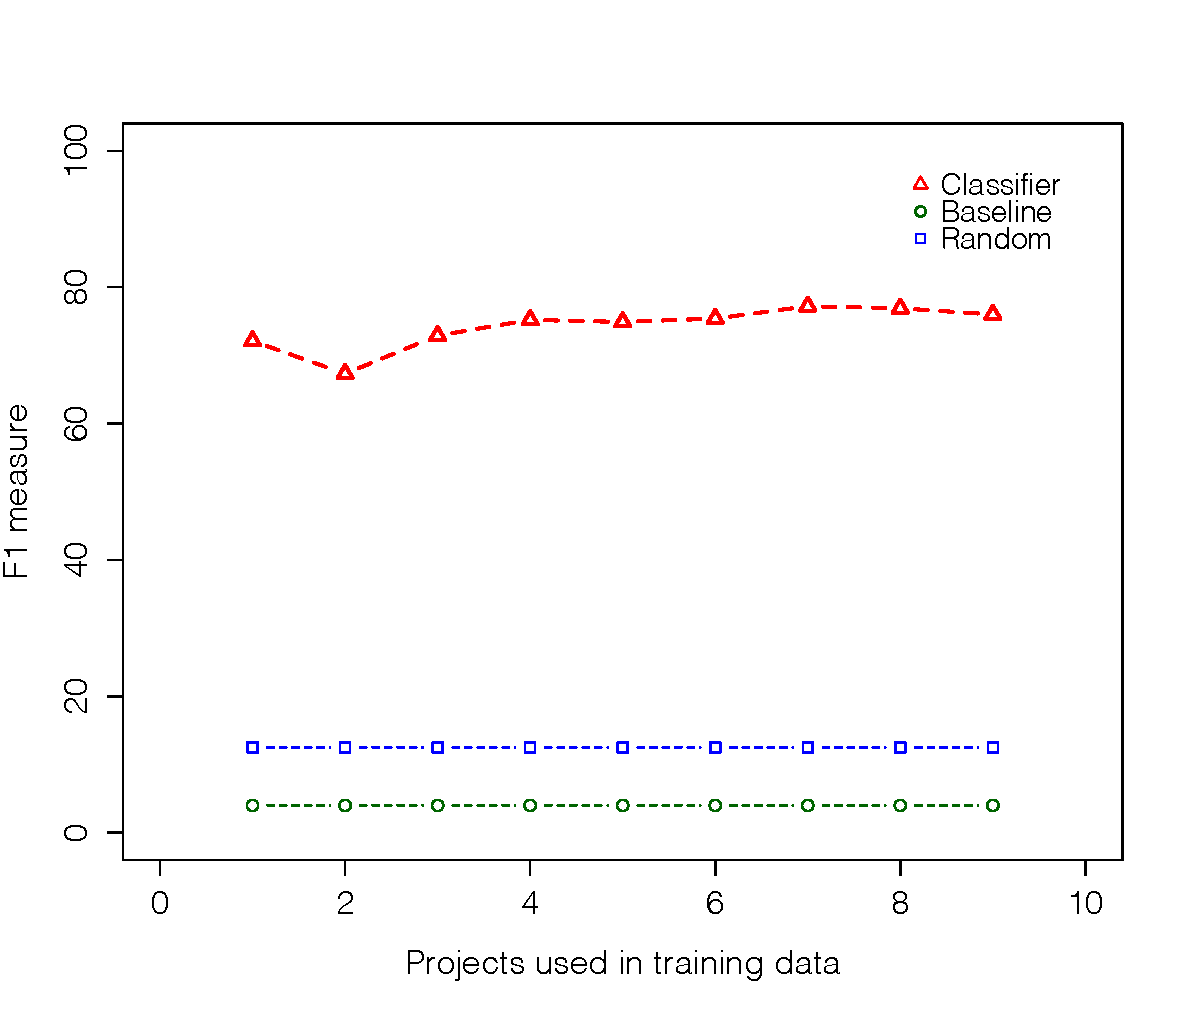
\includegraphics[width = 0.48\textwidth]{figures/implementation_argo.pdf}
  \vspace{-3mm}
  \caption{ArgoUml Requirement Debt classification}
  \label{fig:implementation_argo_result}
\end{figure}

For requirement \SATD comments we find that although there is variation in the F1 measure value during the first 3 iterations they are not so preeminent as the variation found in design \SATD analysis. The F1 measure in requirement \SATD tend to be more constant through the iterations, and the first iteration has already a high percentage of the maximum F1 measured achieved for each project. Figure \ref{fig:implementation_argo_result} shows the evolution of the F1 measure over the iterations for requirement \SATD identification in ArgoUml. 

The values of the F1 measure shown In Figure \ref{fig:implementation_argo_result} are in order execution: 0.721, 0.673, 0.729, 0.752, 0.749, 0.754, 0.772, 0.769 and 0.760.

ArgoUML has F1 measure of 0.721 during the first iteration, 0.729 in the third iteration and 0.772 in the seventh iteration which was the highest F1 measure achieved. The improvement in the F1 measure between the first and third iteration is very low as it is between the fourth and the sixth iteration. In the first iteration the classifier was trained with 150 requirement \SATD comments, which means 27\% of the comments that where used in the ninth iteration. A reduction of 73\% of the necessary training data to achieve almost the same result in terms of F1 measure in this case. 

We analyzed the average percentage of the maximum F1 measure while identifying requirement \SATD comments. The seventh iteration was the one with highest average percentage of the maximum F1 measure achieving a value of 89.89\%. In the seventh iteration an average of 1,055 requirement \SATD comments were used in the training dataset representing 97\% of all requirement \SATD comments that we classified during this study.

We find that the first iteration has a hight average of percentage of the maximum F1 across all projects (i.e., 83\%). Although this percentage still lower than the achieved at the seventh iteration (i.e., 88\%), the training dataset used an average of 600 \SATD comments representing a reduction of 44\% in the necessary comments to create an effective training dataset to classify requirement \SATD comments. Table \ref{tbl:requirement_iteration_performance} shows the average maximum F1 measure for each iteration. 

\begin{table}[!thb]
    \begin{center}
        \caption{Average maximum F1 measure for Design Debt}
        \label{tbl:design_iteration_performance}
        \begin{tabular}{l| c c }
        \toprule
        \thead{Iteration\\Number} & \thead{\% of maximum\\F1 measure} & \thead{Average\\comments} \\
        \midrule
         1  &  0.684  & 756   \\  
         2  &  0.805  & 1,106 \\  
         3  &  0.863  & 1,444 \\  
         4  &  0.879  & 1,717 \\  
         5  &  0.857  & 1,919 \\  
         6  &  0.931  & 2,108 \\  
         7  &  0.950  & 2,251 \\  
         8  &  0.958  & 2,353 \\  
         9  &  0.966  & 2,432 \\  
        \bottomrule
        \end{tabular}
    \end{center}    
\end{table}

\begin{table}[!thb]
	\begin{center}
		\caption{Average maximum F1 measure for Requirement Debt}
		\label{tbl:requirement_iteration_performance}
		\begin{tabular}{l| c c }
			\toprule
			\thead{Iteration\\Number} & \thead{\% of maximum\\F1 measure} & \thead{Average\\comments} \\
			\midrule
			1  &  0.684  & 756 \\  
			2  &  0.805  & 1,106 \\  
			3  &  0.863  & 1,444 \\  
			4  &  0.879  & 1,717 \\  
			5  &  0.857  & 1,919 \\  
			6  &  0.931  & 2,108 \\  
			7  &  0.950  & 2,251 \\  
			8  &  0.958  & 2,353 \\  
			9  &  0.966  & 2,432 \\  
			\bottomrule
		\end{tabular}
	\end{center}    
\end{table}

During the execution of the experiment we notice that the classification can vary accordingly with the project being classified and the data used as test. We also intuitively know that developers from different projects express them selfs differently. These characteristics can be observed during the iterative classification where the addition of more comments not necessarily implies in a improvement on the F1 measure.

One of the reasons for this is that the weight of features is given trough empirical probability, and consequently features that appears with more frequency will have a higher weight. Although this is an effective process for the majority of cases that we studied, it can be misleading when classifying comments that has different context. With smaller datasets such as the training data for requirement \SATD, the addition of comments that does not represent the way that developers write comments in the classified project will actually decrease the F1 measure performance. 

\conclusionbox{We find that the design \SATD comments can be classified effectively using a training dataset of 1,444 these comments. Similarly requirement \SATD can be classified building a training dataset with 1,055 comments of this category.}